\documentclass[fleqn]{article}
\usepackage[utf8]{inputenc}
\usepackage[letterpaper,margin=1in]{geometry}
\usepackage{graphicx}
\usepackage[per-mode=symbol]{siunitx}
\usepackage{amsmath}
\usepackage{float}
\usepackage{listings}
\usepackage{matlab-prettifier}

\title{Homework 4\\ENERGY 293}
\author{Gabriel Buchsbaum}

\begin{document}
\lstset{language=Matlab}

\maketitle

\section{Equations}

\subsection{Electrical model}

\begin{figure}[htb]
\begin{center}
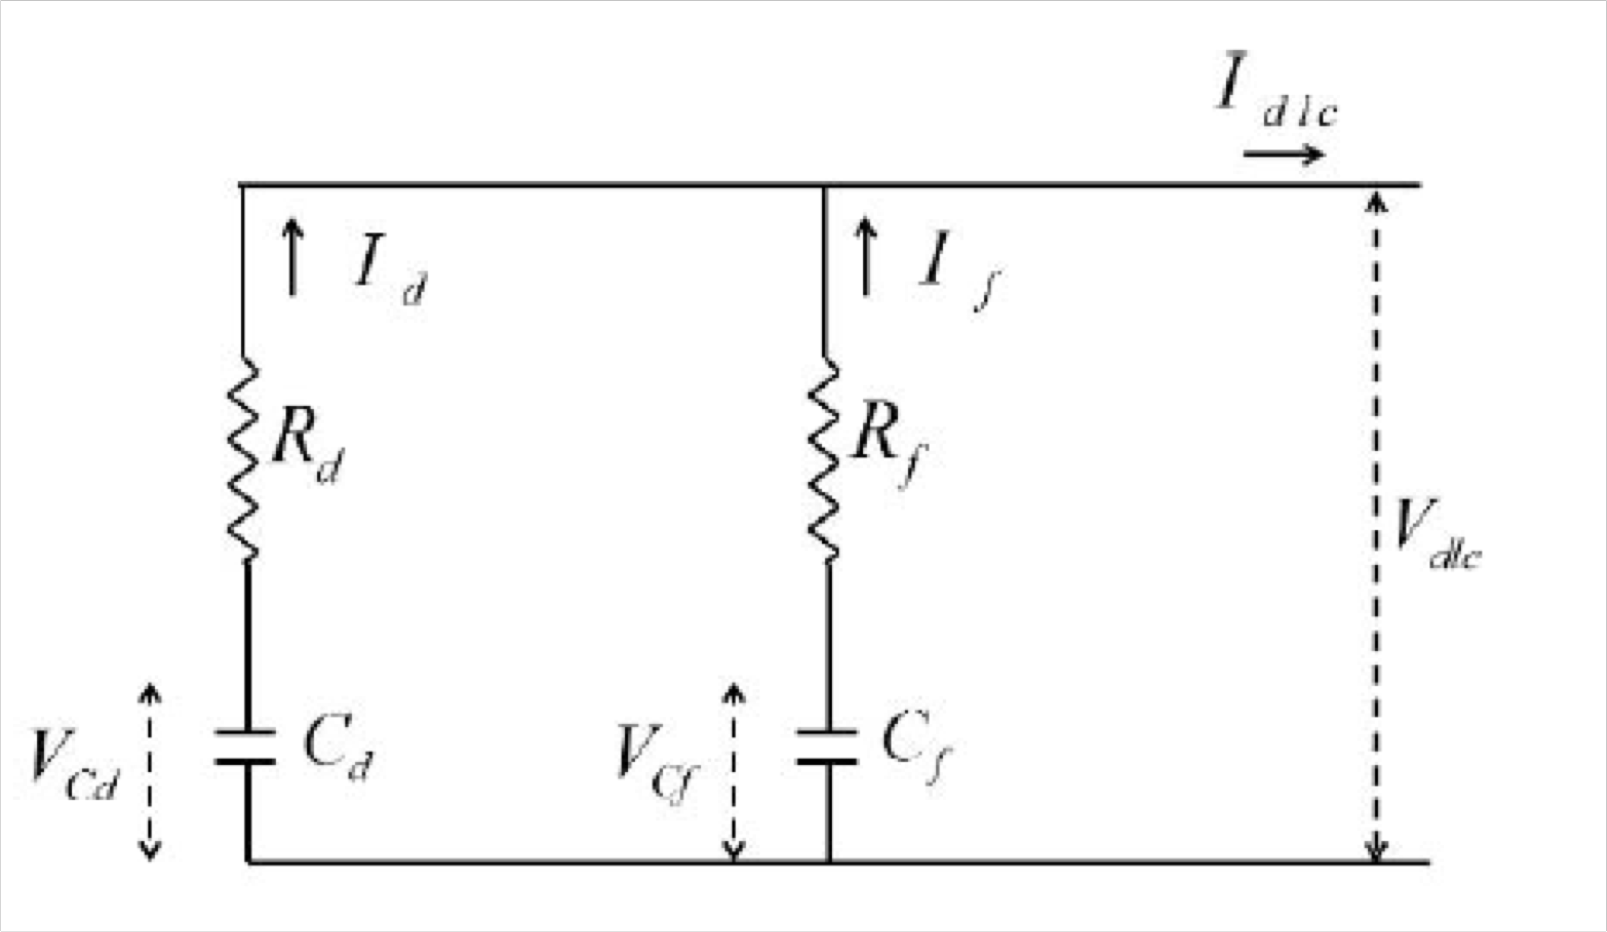
\includegraphics[width=0.75\linewidth]{circuit.png}
\caption{Equivalent circuit diagram (image from assignment)}
\label{fig:circuit}
\end{center}
\end{figure}

From Kirchoff's current law:
\begin{equation}
I_{dlc} = I_f + I_d
\label{eqn:kcl}
\end{equation}

From Kirchoff's voltage law:\footnote{Using convention that positive current is discharging and negative current is charging. This is the convention implied by the circuit diagram and used in the temperature equations and example cycling plot, but is the opposite of the convention used in the equations from lecture notes.}
\begin{equation}
V_{dlc} = V_{cf} - I_f R_f = V_{cd} - I_d R_d
\label{eqn:kvl}
\end{equation}

From the defined behavior of a capacitor:
\begin{equation}
\dot{V}_{cf} = \frac{I_f}{C_f}
\label{eqn:dVcf}
\end{equation}
\begin{equation}
\dot{V}_{cd} = \frac{I_d}{C_d}
\label{eqn:dVcd}
\end{equation}

Rearranging Equation \ref{eqn:kcl}:
\begin{equation}
I_f = I_{dlc} - I_d
\label{eqn:If}
\end{equation}

Substituting Equation \ref{eqn:If} into Equation \ref{eqn:kvl}:
\begin{equation}
V_{dlc} = V_{cf} - \left(I_{dlc} - I_d\right) R_f = V_{cd} - I_d R_d
\label{eqn:kvl2}
\end{equation}

Solving Equation \ref{eqn:kvl2} for $I_d$:
\begin{equation}
V_{cf} - I_{dlc} R_f + I_d R_f = V_{cd} - I_d R_d
\end{equation}
\begin{equation}
I_d \left(R_f + R_d\right) = I_{dlc} R_f + V_{cd} - V_{cf}
\end{equation}
\begin{equation}
I_d = \frac{I_{dlc} R_f + V_{cd} - V_{cf}}{R_f + R_d}
\label{eqn:Id}
\end{equation}

At each time instant, $V_{cf}$, $V_{cd}$, and $I_{dlc}$ are known, and parameters $R_f.$, $R_d$, $C_f$, and $C_d$ are given at the current temperature.  Thus, the following process is used to determine $\dot{V}_{cf}$ and $\dot{V}_{cd}$:
\begin{enumerate}
\item Calculate $I_d$ using Equation \ref{eqn:Id}
\item Calculate $I_f$ using Equation \ref{eqn:If}
\item Calculate $\dot{V}_{cf}$ and $\dot{V}_{cd}$ using Equations \ref{eqn:dVcf} and \ref{eqn:dVcd}
\end{enumerate}

The combined equations are:
\begin{equation}
\dot{V}_{cf} = \frac{I_{dlc} R_d + V_{cf} - V_{cd}}{C_f R_f + C_f R_d}
\label{eqn:dVcf2}
\end{equation}
\begin{equation}
\dot{V}_{cd} = \frac{I_{dlc} R_f + V_{cd} - V_{cf}}{C_d R_f + C_d R_d}
\label{eqn:dVcd2}
\end{equation}

\subsection{Thermal model}

From the lecture slides:
\begin{equation}
\dot{Q}_{gen} = 
\begin{cases}
i_{dlc}^2 R & i_{dlc} > 0 \\
i_{dlc}^2 R - i_{dlc} v_{dlc} \left(1 - \eta\right) & i_{dlc} < 0
\end{cases}
\label{eqn:qgen}
\end{equation}

\begin{equation}
C_{th} \dot{T}_{dlc} + \frac{1}{R_{th}} T_{dlc} = \frac{1}{R_{th}} T_{air} + \dot{Q}_{gen}
\label{eqn:thermal}
\end{equation}

For Equation \ref{eqn:qgen}, the value of $v_{dlc}$ can be determined using Equation \ref{eqn:kvl} and the current $V_{cf}$, $V_{cd}$, and $I_{dlc}$.

Solving Equation \ref{eqn:thermal} for $\dot{T}_{dlc}$:
\begin{equation}
\dot{T}_{dlc} = \frac{\frac{T_{air}}{R_{th}} + \dot{Q}_{gen} - \frac{T_{dlc}}{R_{th}}}{C_{th}}
\label{eqn:dTdlc}
\end{equation}

Equations \ref{eqn:qgen} and \ref{eqn:dTdlc} can be combined into
\begin{equation}
\dot{T}_{dlc} = 
\begin{cases}
\frac{\frac{T_{air}}{R_{th}} + i_{dlc}^2 R - \frac{T_{dlc}}{R_{th}}}{C_{th}} & i_{dlc} > 0 \\
\frac{\frac{T_{air}}{R_{th}} + i_{dlc}^2 R - i_{dlc} v_{dlc} \left(1 - \eta\right) - \frac{T_{dlc}}{R_{th}}}{C_{th}} & i_{dlc} < 0
\end{cases}
\label{eqn:dTdlc2}
\end{equation}

These two models can be solved simultaneously in the same ODE function. Since the ode45 solver provides the current values of $V_{cf}$, $V_{cd}$, and $T_{dlc}$, and can also use a given $I_{dlc}$ and $T_{air}$, all that needs to be done is determine the values of the electrical parameters at the current $T_{dlc}$ and return the results of Equations \ref{eqn:dVcf2}, \ref{eqn:dVcd2}, and \ref{eqn:dTdlc2}

\section{Matlab code}

\begin{lstlisting}[style=Matlab-editor]
% Eliminate all extraneous variables and plots
close all
clearvars

% First run with air temperature of 0 C
Tair = 0;
% Set initial conditions
IC = [0, 0, Tair];
% Generate 50 seconds of rest before first cycle
Idlc = 0;
[t0, V0] = ode45(@(t, V)odefcn(t, V, Idlc, Tair), [-50, 0], IC);
I0 = zeros(length(t0),1);
% t0, V0, and I0 refer to time, differential equation results, and 
% current at 0 C. They are constantly added to in each cycle.

% Run 5 cycles
for i = 1:5
    % Start with charging art of cycle
    Idlc = -100;
    % Use event function to stop when Vdlc reaches rated voltage.
    % The anonymous function @(t, V)event(t,V,Idlc) allows ode45
    % to interpret using it as a function of t and V, while still
    % using Idlc to calculate Vdlc.
    options = odeset('Events',@(t, V)event(t,V,Idlc));
    % Gain initial conditions from end of V0
    IC = V0(length(t0),:);
    % Run from last time value to arbitrary large time.
    % The event function should stop it well before this time.
    tRange = [max(t0),1000000];
    % Run ode45 solver on this part of the cycle. The anonymous
    % function @(t,V)odefcn(t,V,Idlc,Tair) allows ode45 to interpret
    % the ODE function as a function of just t and V, while still
    % using the Idlc and Tair parameters.
    [t1,V1] = ode45(@(t,V)odefcn(t,V,Idlc,Tair), tRange, IC, options);
    % Store array of current values
    I1 = zeros(length(t1),1) + Idlc;
    
    % Continue with first resting step
    Idlc = 0;
    % Initial conditions are from the end of charging
    IC = V1(length(t1),:);
    % Go from end of charging to 15 seconds past it
    tRange = [max(t1), max(t1)+15];
    [t2,V2] = ode45(@(t,V)odefcn(t,V,Idlc,Tair), tRange, IC);
    % Store array of current values
    I2 = zeros(length(t2),1);
    
    % Discharge step
    Idlc = 100;
    % Refresh event function with new current
    options = odeset('Events',@(t, V)event(t,V,Idlc));
    % Initial conditions taken from end of rest
    IC = V2(length(t2),:);
    % Run from end of rest to arbitrary large time.
    % The event function should stop it well before this time.
    tRange = [max(t2),1000000];
    [t3,V3] = ode45(@(t,V)odefcn(t,V,Idlc,Tair), tRange, IC, options);
    % Store array of current values
    I3 = zeros(length(t3),1) + Idlc;
    
    % Second resting step
    Idlc = 0;
    % Initial conditions are from the end of discharging
    IC = V3(length(t3),:);
    % Go from end of discharge to 15 seconds past it
    tRange = [max(t3), max(t3)+15];
    [t4, V4] = ode45(@(t, V)odefcn(t, V, Idlc, Tair), tRange, IC);
    % Store array of current values
    I4 = zeros(length(t4),1);
    
    % Concatenate the results to the t0, V0, and I0 arrays
    t0 = vertcat(t0, t1, t2, t3, t4);
    V0 = vertcat(V0, V1, V2, V3, V4);
    I0 = vertcat(I0, I1, I2, I3, I4);
end

% Go through each time value and calculate the Vdlc at that time
Vdlc0 = zeros(length(t1), 1);
for i = 1:length(t0)
    Vdlc0(i) = voltage(V0(i,:), I0(i));
end

% Repeat process with air temperature of 40 C
Tair = 40;
IC = [0, 0, Tair];

Idlc = 0;
[t40, V40] = ode45(@(t, V)odefcn(t, V, Idlc, Tair), [-50, 0], IC);
I40 = zeros(length(t40),1);

for i = 1:5
    Idlc = -100;
    options = odeset('Events',@(t, V)event(t,V,Idlc));
    IC = V40(length(t40),:);
    tRange = [max(t40),1000000];
    [t1,V1] = ode45(@(t,V)odefcn(t,V,Idlc,Tair), tRange, IC, options);
    I1 = zeros(length(t1),1) + Idlc;
    
    Idlc = 0;
    IC = V1(length(t1),:);
    tRange = [max(t1), max(t1)+15];
    [t2, V2] = ode45(@(t, V)odefcn(t, V, Idlc, Tair), tRange, IC);
    I2 = zeros(length(t2),1);
    
    Idlc = 100;
    options = odeset('Events',@(t, V)event(t,V,Idlc));
    IC = V2(length(t2),:);
    tRange = [max(t2),1000000];
    [t3,V3] = ode45(@(t,V)odefcn(t,V,Idlc,Tair), tRange, IC, options);
    I3 = zeros(length(t3),1) + Idlc;
    
    Idlc = 0;
    IC = V3(length(t3),:);
    tRange = [max(t3), max(t3)+15];
    [t4, V4] = ode45(@(t, V)odefcn(t, V, Idlc, Tair), tRange, IC);
    I4 = zeros(length(t4),1);
    
    t40 = vertcat(t40, t1, t2, t3, t4);
    V40 = vertcat(V40, V1, V2, V3, V4);
    I40 = vertcat(I40, I1, I2, I3, I4);
end

Vdlc40 = zeros(length(t1), 1);
for i = 1:length(t40)
    Vdlc40(i) = voltage(V40(i,:), I40(i));
end

% Plot and save results
% Vdlc at 0 C
figure
yyaxis left
plot(t0, I0)
ylim([-160,160])
xlabel("Time (s)")
ylabel("Current (A)")
grid on
yyaxis right
plot(t0,Vdlc0)
ylim([-0.1,3.1])
ylabel("Voltage (V)")
saveas(gcf,'Vdlc_0.png')
% Voltage at 40 C
figure
yyaxis left
plot(t40, I40)
ylim([-160,160])
xlabel("Time (s)")
ylabel("Current (A)")
grid on
yyaxis right
plot(t40,Vdlc40)
ylim([-0.1,3.1])
ylabel("Voltage (V)")
saveas(gcf,'Vdlc_40.png')
% Temperature at 0 C
figure
yyaxis left
plot(t0, I0)
ylim([-160, 160])
xlabel("Time (s)")
ylabel("Current (A)")
grid on
yyaxis right
plot(t0,V0(:,3))
ylim([-0.4, 12.4])
ylabel("Temperature (C)")
saveas(gcf,'Tdlc_0.png')
% Temperature at 40 C
figure
yyaxis left
plot(t40,I40)
ylim([-160, 160])
xlabel("Time (s)")
ylabel("Current (A)")
grid on
yyaxis right
plot(t40,V40(:,3))
ylim([39.6, 52.4])
ylabel("Temperature (C)")
saveas(gcf,'Tdlc_40.png')

% ODE function to determine how Vcf, Vcd, and Tdlc change.
% It takes in a time value, an array containing the Vcf, Vcd,
% and Tdlc, Idlc, and Tair. It returns a vertical array showing
% the derivatives of Vcf, Vcd, and Tdlc.
function dVdt = odefcn(t, V, Idlc, Tair)
Vcf = V(1);
Vcd = V(2);
Tdlc = V(3);
% Obtain electrical parameters at the current temperature
[Rd, Rf, Cd, Cf] = Eparams(Tdlc);
% Solve for Id and If
Id = (Idlc * Rf - Vcf + Vcd) / (Rd + Rf);
If = Idlc - Id;
% Solve for derivatives of Vcf and Vcd
dVcf = -If / Cf;
dVcd = -Id / Cd;
% Obtain temperature parameters
[R, eta, Rth, Cth] = Tparams;
% Determine heat generated
if Idlc >= 0 % if discharging
    Qgen = Idlc^2 * R;
else % if charging
    Qgen = Idlc^2 * R - Idlc * voltage(V, Idlc) * (1 - eta);
end
% Solve for derivative of temperature
dTdlc = (Tair / Rth + Qgen - Tdlc / Rth) / Cth;
% Place derivatives in vertical array to return
dVdt = [dVcf; dVcd; dTdlc];
end

% Event function to stop charge and discharge cycles
function [ev,s,dir] = event(t, V, Idlc)
% Determine Vdlc
Vdlc = voltage(V, Idlc);
% Trigger when Vdlc is rated voltage or half rated voltage
ev = [Vdlc - 2.7; Vdlc - 1.35];
% Stop in both cases
s = [1; 1];
% Only trigger when rising to 2.7V or falling to 1.35V
dir = [1; -1];
end

% Function to calculate Vdlc with given Vcf, Vcd, and Idlc
function Vdlc = voltage(V, Idlc)
Vcf = V(1);
Vcd = V(2);
Tdlc = V(3);
% Obtain electrical parameters at current temperature
[Rd, Rf, Cd, Cf] = Eparams(Tdlc);
% Split Idlc into Id and If
Id = (Idlc * Rf - Vcf + Vcd) / (Rd + Rf);
% Calculate Vdlc
Vdlc = -Id * Rd + Vcd;
end

% Function to determine electrical parameters at a given temperature
function [Rd, Rf, Cd, Cf] = Eparams(Tdlc)
% Take parameter values at each temperature and interpolate
Rd = interp1([-18, 25, 50], [0.238, 0.287, 0.226], Tdlc);
Rf = interp1([-18, 25, 50], [0.549, 0.533, 0.496], Tdlc)*10^-3;
Cd = interp1([-18, 25, 50], [64.3, 64.3, 112.1], Tdlc);
Cf = interp1([-18, 25, 50], [1355, 1368, 1481], Tdlc);
end

% Function to store temperature parameters (to keep in one location)
function [R, eta, Rth, Cth] = Tparams
R = 0.00047;
eta = 0.9;
Rth = 4.5;
Cth = 320;
end
\end{lstlisting}

\pagebreak

\section{Results}

\begin{figure}[!htb]
\begin{center}
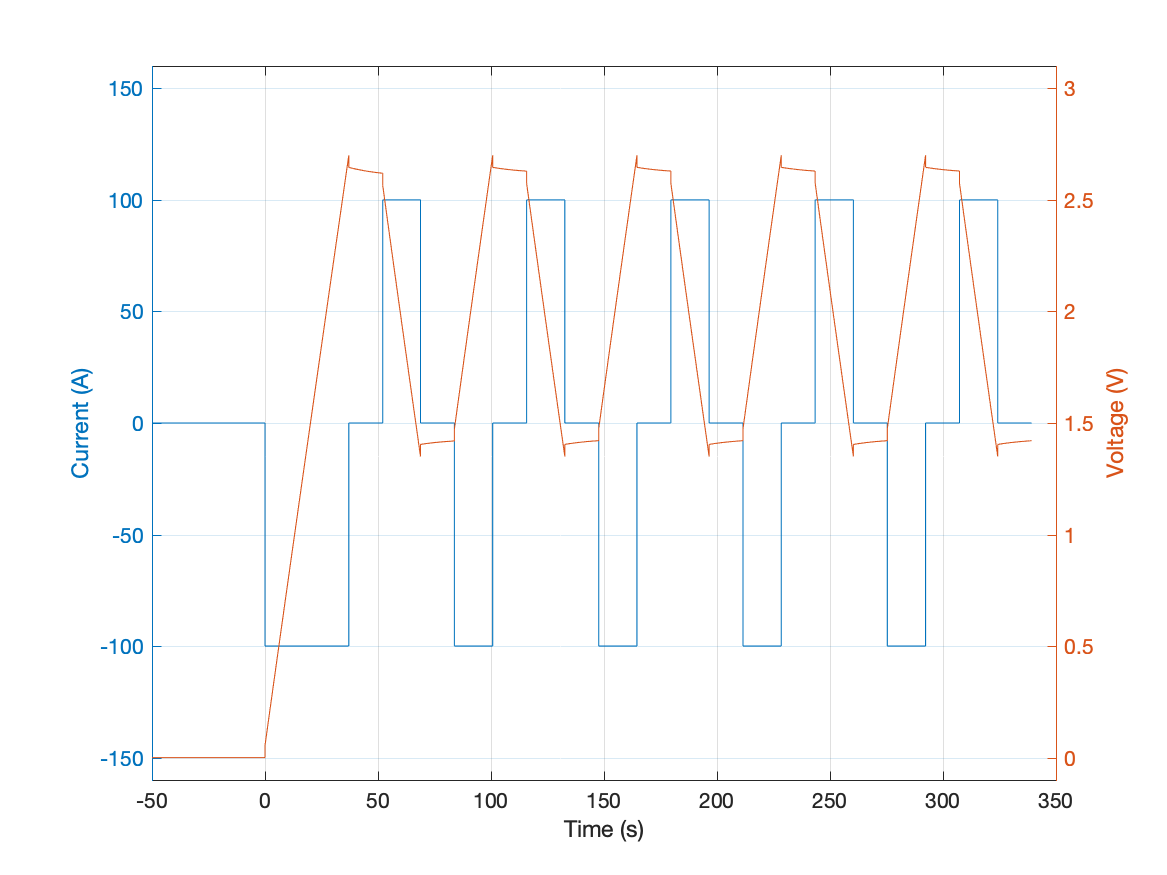
\includegraphics[width=0.73\linewidth]{Vdlc_0.png}
\caption{$V_{dlc}$ under given cycling with $T_{air}$ of \SI{0}{\celsius}}
\label{fig:Vdlc0}
\end{center}
\end{figure}

\begin{figure}[!htb]
\begin{center}
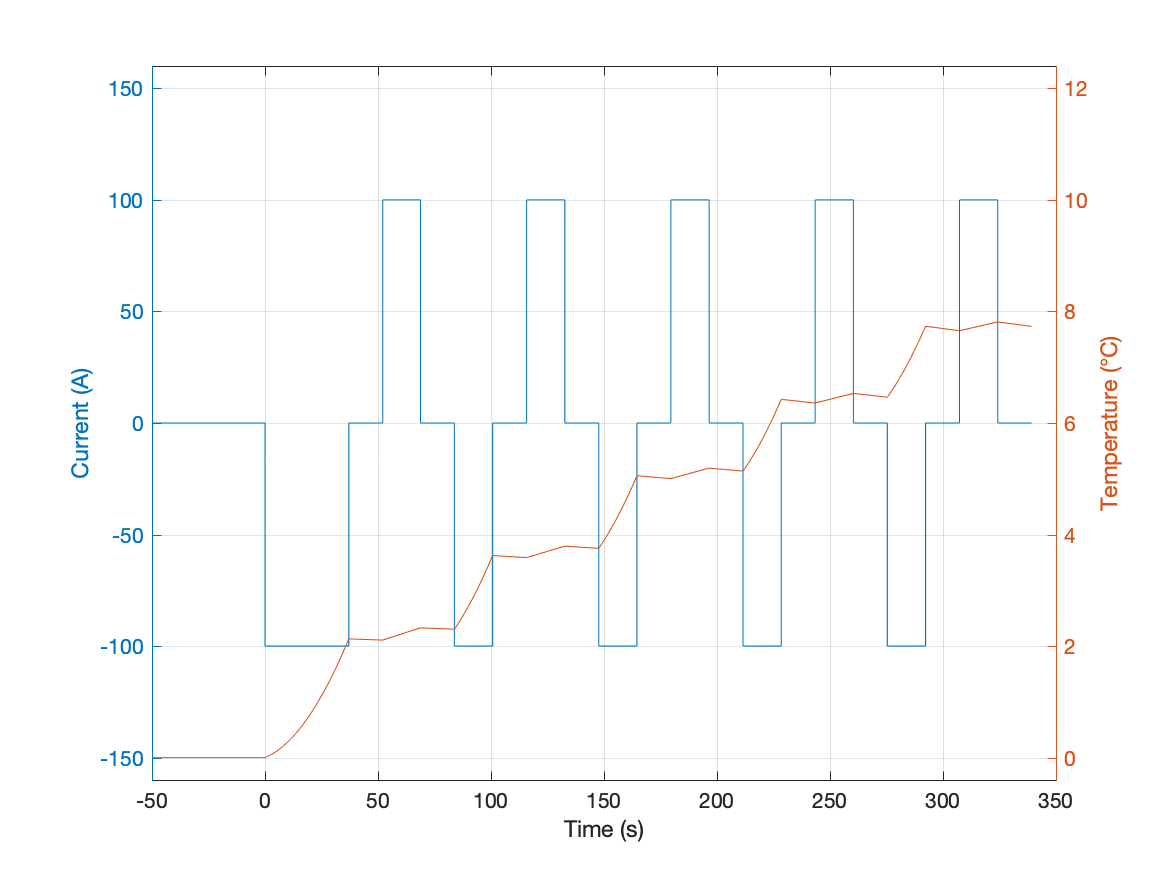
\includegraphics[width=0.73\linewidth]{Tdlc_0.png}
\caption{$T_{dlc}$ under given cycling with $T_{air}$ of \SI{0}{\celsius}}
\label{fig:Tdlc0}
\end{center}
\end{figure}

\begin{figure}[!htb]
\begin{center}
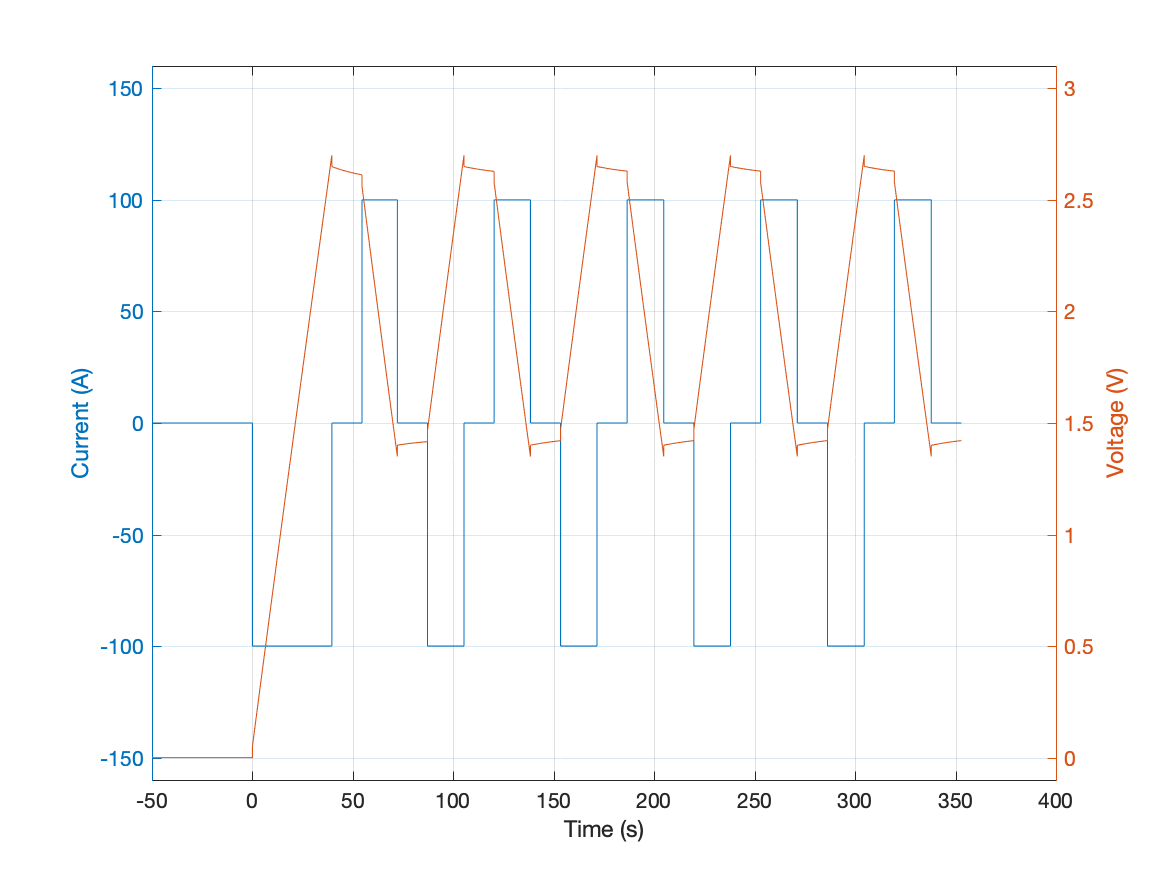
\includegraphics[width=0.76\linewidth]{Vdlc_40.png}
\caption{$V_{dlc}$ under given cycling with $T_{air}$ of \SI{40}{\celsius}}
\label{fig:Vdlc40}
\end{center}
\end{figure}

\begin{figure}[!htb]
\begin{center}
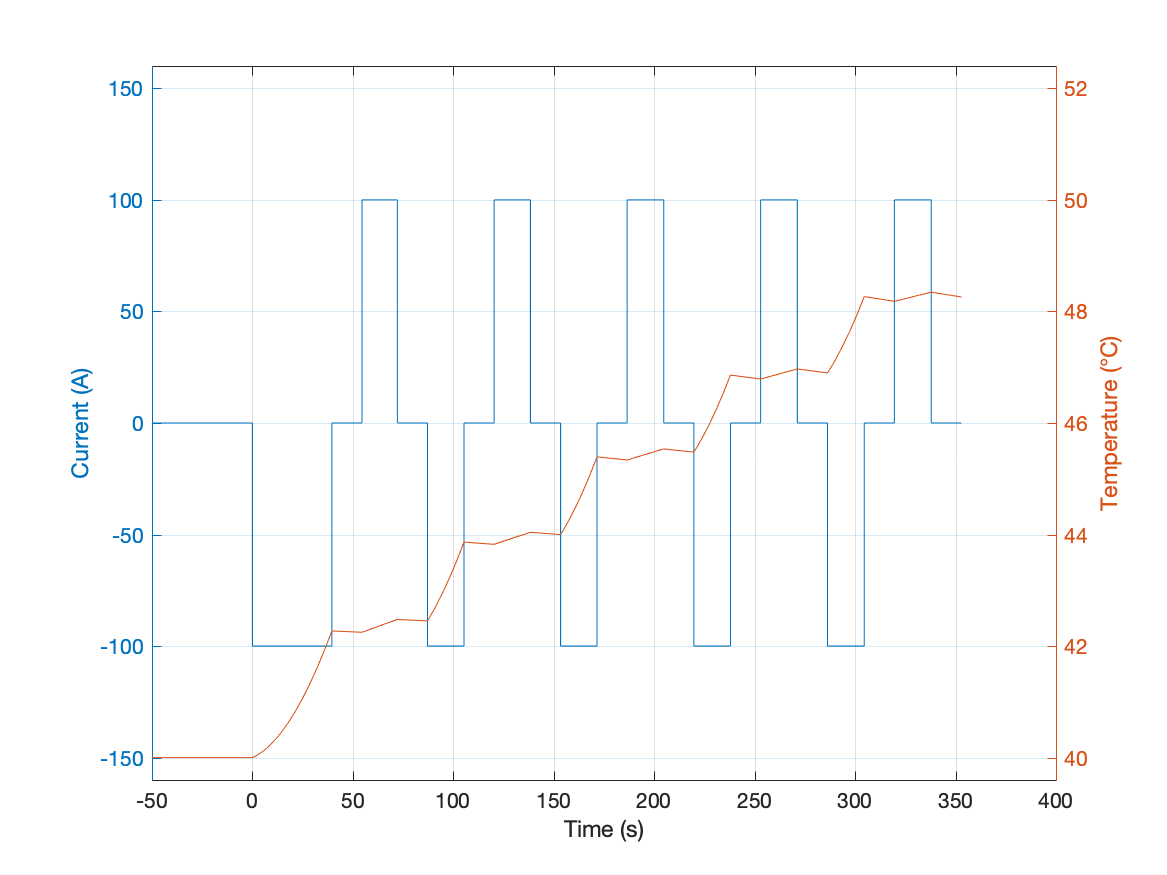
\includegraphics[width=0.76\linewidth]{Tdlc_40.png}
\caption{$T_{dlc}$ under given cycling with $T_{air}$ of \SI{40}{\celsius}}
\label{fig:Tdlc40}
\end{center}
\end{figure}

As Figures \ref{fig:Vdlc0} and \ref{fig:Vdlc40} show, the voltage change is effectively linear when charging and discharging the capacitor. When the capacitor is at rest, the voltage increases or decreases somewhat due to charge moving between $C_f$ and $C_d$.  There is a jump in voltage at the beginning and end of each phase caused by the amount of current flowing through $R_f$ and $R_d$ changing dramatically.

As Figures \ref{fig:Tdlc0} and \ref{fig:Tdlc40} show, the temperature always rises when the capacitor is charging or discharging, but rises faster when charging than discharging.  The temperature decreases slightly towards toom temperature during resting periods, but not enough to overcome the increase during the rest of the cycle.

There is no particularly significant difference between the supercapacitor behavior at \SI{0}{\celsius} and \SI{40}{\celsius}.  Voltage change is slightly slower at the higher temperature, but the difference is minimal. Also, the temperature rise is greater at the higher temperature, most likely due to the longer time that the supercapacitor is drawing current or having current drawn from it.

\end{document}